\newcommand{\subject}{BPC-TIN}
\newcommand{\subjectname}{Teoretická informatika}
% Pokud jste přidali otázku nebo její část, přidejte své jméno sem
\newcommand{\authors}{kámen u~cesty}
% Pokud jste opravili gramatickou, logickou nebo formátovací chybu, přidejte své jméno sem
\newcommand{\corrections}{kámen u~cesty, czechbol}

% FEKT.tex
% https://github.com/VUT-FEKT-IBE/FEKT.tex
% Git hash repozitáře v době kopírování: 35133a18ec74b314184f538e33c7f92054123d09

\documentclass[
    % Velikost základního písma je 12 bodů
    12pt,
    % Formát papíru je A4
    a4paper,
    % Oboustranný tisk
    twoside,
    % Záložky a metainformace ve výsledném PDF budou v kódování unicode
    unicode,
]{article}

%%%%%%%%%%%%%%%%%%%%
% OBECNÉ NASTAVENÍ %
%%%%%%%%%%%%%%%%%%%%

% Kódování zdrojových souborů
\usepackage[utf8]{inputenc}
% Kódování výstupního souboru
\usepackage[T1]{fontenc}
% Podpora češtiny
\usepackage[czech]{babel}

% Geometrie stránky
\usepackage[
    % Horní a dolní okraj
    tmargin=25mm,
    bmargin=25mm,
    % Vnitřní a vnější okraj
    lmargin=30mm,
    rmargin=20mm,
    % Velikost zápatí
    footskip=17mm,
    % Vypnutí záhlaví
    nohead,
]{geometry}

% Zajištění kopírovatelnosti a prohledávanosti vytvořených PDF
\usepackage{cmap}
% Podmínky (pro použití v titulní straně)
\usepackage{ifthen}

%%%%%%%%%%%%%%%
% FORMÁTOVÁNÍ %
%%%%%%%%%%%%%%%

% Nastavení stylu nadpisů
\usepackage{sectsty}
% Formátování obsahů
\usepackage{tocloft}
\setcounter{tocdepth}{1}
% Odstranění mezer mezi řádky v seznamech
\usepackage{enumitem}
\setlist{nosep}
\setitemize{leftmargin=1em}
\setenumerate{leftmargin=1.5em}
\renewcommand{\labelitemi}{--}
\renewcommand{\labelitemii}{--}
\renewcommand{\labelitemiii}{--}
\renewcommand{\labelitemiv}{--}
% Sázení správných uvozovek pomocí '\enquote{}'
\usepackage{csquotes}
% Vynucení umístění poznámek pod čarou vespod stránky
\usepackage[bottom]{footmisc}
% Automatické zarovnání textu k předcházení vdov a parchantů
\usepackage[defaultlines=3,all=true]{nowidow}
% Zalomení části textu pokud není na současné stránce dost místa
\usepackage{needspace}
% Nastavení řádkování
\usepackage{setspace}
\onehalfspacing
% Změna odsazení odstavců
\setlength{\parskip}{1em}
\setlength{\parindent}{0em}

% Bezpatkové sázení nadpisů
\allsectionsfont{\sffamily}
% Změna formátování nadpisu a podnadpisů v Obsahu
\renewcommand{\cfttoctitlefont}{\Large\bfseries\sffamily}
\renewcommand{\cftsubsecdotsep}{\cftdotsep}

% Použití moderní/aktualizované sady písem
\usepackage{lmodern}

%%%%%%%%%%%
% NADPISY %
%%%%%%%%%%%

\usepackage{titlesec}

\titlespacing*{\section}{0pt}{10pt}{-0.2\baselineskip}
\titlespacing*{\subsection}{0pt}{0.2\baselineskip}{-0.2\baselineskip}
\titlespacing*{\subsubsection}{0pt}{0.2\baselineskip}{-0.2\baselineskip}
\titlespacing*{\paragraph}{0pt}{0pt}{1em}

%%%%%%%%%%
% ODKAZY %
%%%%%%%%%%

% Tvorba hypertextových odkazů
\usepackage[
    breaklinks=true,
    hypertexnames=false,
]{hyperref}
% Nastavení barvení odkazů
\hypersetup{
    colorlinks,
    citecolor=black,
    filecolor=black,
    linkcolor=black,
    urlcolor=blue
}

%%%%%%%%%%%%%%%%%%%%%%%%%%%
% OBRÁZKY, GRAFY, TABULKY %
%%%%%%%%%%%%%%%%%%%%%%%%%%%

% Vkládání obrázků
\usepackage{graphicx}
\usepackage{subfig}
% Nastavení popisů obrázků, výpisů a tabulek
\usepackage{caption}
\captionsetup{justification=centering}
% Grafy a vektorové obrázky
\usepackage{tikz}
\usetikzlibrary{shapes,arrows}
% Složitější tabulky
\usepackage{tabularx}
\usepackage{multicol}

% Sázení osamocených float prostředí v horní části stránky
\makeatletter
\setlength{\@fptop}{0pt plus 10pt minus 0pt}
\makeatother

% Vynucení vypsání floating prostředí pomocí \FloatBarrier
\usepackage{placeins}

%%%%%%%%%%%%%%
% MATEMATIKA %
%%%%%%%%%%%%%%

% Sázení matematiky a matematických symbolů ('\mathbb{}')
\usepackage{amsmath}
\usepackage{amssymb}
% Sázení fyzikálních veličin
\usepackage{siunitx}

%%%%%%%%%%%%%%%%%
% ZDROJOVÉ KÓDY %
%%%%%%%%%%%%%%%%%

% Sazba zdrojových kódů
\usepackage[formats]{listings}
% Přepnutí prostředí 'code' do režimu výpisu kódu
\newenvironment{code}{\captionsetup{type=listing}}{}

% Balíček 'minted' budeme používat pouze pokud je jeho hodnota nastavena na 'true'
\providecommand{\docminted}{false}
\ifthenelse{\equal{\docminted}{true}}
{
    % Sazba zdrojových kódů
    \usepackage[newfloat]{minted}
    % Nastavení barev 'minted' kódů
    \usemintedstyle{pastie}
}
{
    % \docminted není 'true', nic neprovádíme
    % Pokud je v dokumentu 'minted' prostředí, dokument se nepodaří přeložit.
}

%%%%%%%%%%%
% TITULKA %
%%%%%%%%%%%

\IfFileExists{../.repo.tex}{
    % Soubor '.repo.tex' může (re)definovat povinné a nepovinné argumenty
    % souboru 'main.tex'. To lze využít v případech kdy v jednom repozitáři
    % existuje více dokumentů najednou (např. státnicové otázky).
    \newcommand{\docdesc}{Otázky ke~státnicím}
\newcommand{\docgroup}{Bakalářský obor Informační bezpečnost, FEKT VUT}
\newcommand{\docurl}{https://github.com/VUT-FEKT-IBE/BPC-IBE-SZZ}

}{}

% Pokud byly nepovinné argumenty zakomentovány nebo vymazány, přidáme prázdné
% definice příkazů, aby bylo dokument možné správně přeložit.
\providecommand{\docdesc}{}
\providecommand{\docgroup}{}
\providecommand{\docurl}{}

\newcommand{\titulka}{
    \vspace*{2em}
    \begin{center}
        {\Huge \bfseries \subject}

        \vspace*{1em}

        {\Huge \bfseries \subjectname}

        \vspace*{2em}

        {\Large \docdesc}

        \vspace*{1em}

        \docgroup

        \url{\docurl}
    \end{center}

    \vfill

    \begin{tabular}{ll}
        Text:      & \authors     \\
        Korektura: & \corrections \\
    \end{tabular}
    \hfill
    \today

    \thispagestyle{empty}
    \newpage
}

\clearpage

\begin{document}

\titulka{}

{
% Speciální úprava aby se Obsah vešel na jednu stranu.
% Když je na stranách dvou, rozbíjí se twopage nebo číslování.
\singlespacing
\tableofcontents
\thispagestyle{empty}
}

\setcounter{page}{0}

\section{Dílčí kroky procesu směrování uvnitř směrovače.}
\begin{itemize}
\item Zpracování příchozích paketů
\begin{itemize}
\item 1. krok
\begin{itemize}
\item Príjem rámca (napr. Ethernet)
\item Na vstupnej časti sieťového rozhrania na úrovni linkovej vrstvy
\begin{itemize}
\item interpretace položek v hlavičce protokolu linkové vrstvy 
\item detekce začátku a konce rámce
\item nakonec - zpracována zapouzdřená datová jednotka (identifikace začátku paketu, identifikace hlavičky paketu )
\end{itemize}
\item Spracovanie na urovni linkovej vrstvy
\begin{itemize}
\item Vyjmutí hlavičky rámce 
\item Vytvorenie kontextu paketu (datová struktura využívaná pro řízení dalších operací ve směrovači) 
\item Vyplnění příslušných polí kontextu paketu
\item Vyjmutí zapouzdřeného paketu a jeho zpracování 
\end{itemize}
\item Zpracování informací síťové vrstvy (L3)
\begin{itemize}
\item Nalezení hlavičky IP
\item Ověření konzistence hlavičky IP
\item Přečtení obsahu IP hlavičky
\item Zápis do kontextu paketu
\end{itemize}
\end{itemize}
\item 2. krok
\begin{itemize}
\item Předání paketu i kontextu do bloku přepojování
\end{itemize}
\item 3. krok
\begin{itemize}
\item Dočasné uložení paketu ve vyrovnávací paměti
\item Vyhledávání v přepojovací tabulce
\item Na základě informací v kontextu paketu
\item Nalezení správného výstupního rozhraní
\item Zápis do kontextu paketu
\end{itemize}
\item 4. krok
\begin{itemize}
\item Předání paketu i kontextu základní desce
\item Plánování přenosu paketu
\item Zohlednění priority paketu
\end{itemize}
\item 5. krok
\begin{itemize}
\item Přenos paketu k odchozímu síťovému rozhraní
\item Postup zpracování na výstupu
\end{itemize}
\end{itemize}


\item Zpracování odchozích paketů
\begin{itemize}
\item 6. krok
\begin{itemize}
\item Předání paketu i kontextu do výstupní linkové karty
\item Uložení paketu ve vyrovnávací paměti
\item Aktualizace adresy v kontextu paketu
\end{itemize}
\item 7. krok
\begin{itemize}
\item Předání kontextu Správě front
\item Kontrola priority paketu (Určené blokem přepojování)
\item Vložení kontextu paketu do odpovídající fronty
\item Naplánování odesílání paketu (Zpravidla podle propustnosti přidělené dané frontě)
\item Zaplnění fronty (Způsobeno zahlcením sítě,riesene Řízenym zahazováním paketů)
\end{itemize}
\item 8. krok
\begin{itemize}
\item Předání paketu i kontextu správě provozu
\item Identifikace uživatele z kontextu
\item Kontrola případného omezení rychlosti pro uživatele
\item Tvarování provozu (Pozdržení paketu, Zahození paketu)
\end{itemize}
\item 9. krok
\begin{itemize}
\item Předání paketu odchozímu síťovému rozhraní
\item Aktualizace informací síťové vrstvy (L3) (Nová hodnota TTL, Výpočet zabezpečení CRC)
\item Vygenerování nové hlavičky linkové vrstvy (L2)
\end{itemize}
\item 10. krok
\begin{itemize}
\item Posledním krokem zpracování paketu je jeho fyzické odeslán
\end{itemize}
\end{itemize}
\end{itemize}
\newpage
\section{Směrovací protokol Distance-Vector, směrovací protokol RIP}
\subsection{Distance-Vector}
Tento typ směrovacích protokolů je založen na distribuovaném výpočtu, v rámci 
kterého každý směrovač spočítá svoji „nejlepší“ cestu k dostupným sítím. Směrovače provádí 
výpočet nezávisle na ostatních. Po skončení výpočtu směrovač informuje svoje sousedy o své 
„nejlepší“ cestě. Na základě těchto informací pak sousední směrovače mohou přehodnotit své 
znalosti o „nejlepších“ cestách. Když sousední směrovač zjistí, že našel „lepší“ cestu, než ta 
původní, tak o tom také informuje svoje sousedy včetně směrovače, od kterého přišla zpráva 
inicializující výpočet. Z popisu je vidět, že stanovení „nejlepší“ cesty je iteračním procesem, 
který probíhá v několika krocích. Mezi klíčové požadavky na tento iterační 
proces patří:
\begin{itemize}
\item Stabilita, tj. aby se proces po konečné době ustálil a nedostal do stavu, kdy si 
směrovače mezi sebou vzájemně cyklicky vyměňují směrovací zprávy.
\item Rychlá konvergence, aby doba potřebná k ustálení byla co nejkratší.
\end{itemize}
\begin{figure}[!h]
  \begin{center}
    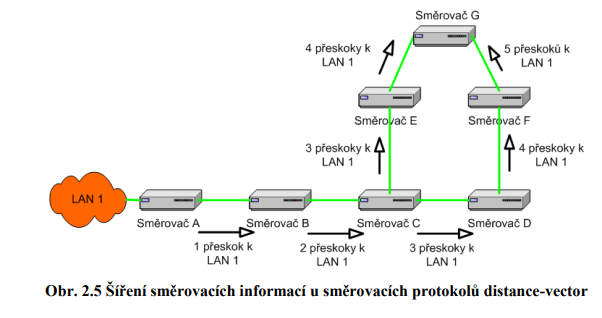
\includegraphics[scale=1]{images/distancevektor.png}
  \end{center}
\end{figure}

„Nejlepší“ cestou v případě směrovacích protokolů distance-vector je považována cesta, 
která obsahuje nejmenší počet přeskoků. Výhodou směrovacích protokolů distance-vector je 
jejich jednoduchá konfigurace, údržba i řešení případných problémů.
Nevýhodou tohoto typu směrovacích protokolů je, že počet přeskoků je často omezen 
na poměrně malou hodnotu (např. 15). Když cílová síť je ve větší vzdálenosti, tak je 
považována za nedostupnou. Dále změna v topologii sítě může způsobit záplavové šíření 
směrovacích informací. Částečnou ochranu proti záplavovému šíření směrovacích informací 
může zajistit omezení rozhraní, přes která směrovač může rozeslat směrovací informace či 
omezení, přes která rozhraní mohou být jaké sítě avizovány. Tato pravidla však musí být 
nakonfigurována ručně. Podporuju agregaciu adries pre lepsiu priehladnost zaznamov v smerovacich tabulbach (spaja suvisle adresne priestory niekolkych podsieti do jedneho velkeho adresne priestoru ktory dalej siri).
\begin{figure}[!h]
  \begin{center}
    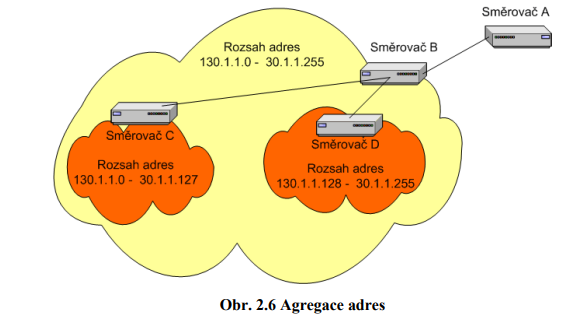
\includegraphics[scale=1]{images/agregacia.png}
  \end{center}
\end{figure}
\subsection{RIP}
Konkrétním představitelem směrovacích protokolů distance-vector je Routing 
Information Protocol (RIP), který je určen především pro využití v lokálních sítích. Iterační proces protokolu je založen na algoritmu označeném jako Ford – Fulkerson či Bellman – Ford. RIP šíří informace o sítích, které zná a dále tyto informace doplňuje o svoji vzdálenost 
od těchto sítí. Maximální vzdálenost je 16 přeskoků. Vzdálenější síť je označena jako 
nedostupná. Vzdálenost přímo připojené sítě je 1 přeskok. Směrovač rozesílá směrovací 
informace po 30 s. Ak neobdrzi spravu z daneho smeru:
\begin{itemize}
\item Po 180 s -> oznaci ako nepouzitelnu
\item Po 240 s -> odstrani zo smerovacej tabulky vsetky info vztahujuce sa k sietam ktore boli dostupne danym smerom
\end{itemize}
RIP v1 nepodporovala masku siete -> neumoznovala delenie adresneho priestoru. RIP v2 uz podporuje. Potenciální problémy, které mohou nastat u tohoto směrovacího protokolu, jsou posílání 
paketů do neplatného směru nebo dlouhá doba konvergence. Tyto problémy se mohou 
projevit např. při kritických událostech, jako je výpadek linky. Tieto problemy sa riesia:
\begin{itemize}
\item Prvním řešením je informovat sousedy o výpadku spojení 
okamžitě místo využití pravidelných aktualizací rozesílaných po 30 s
\item Split Horizon, zakazuje vysílání aktualizací o dané síti po rozhraní, po 
kterém byla informace o této síti přijata. Tato modifikace vyřeší výše popsaný problém, ale 
nedokáže eliminovat problémy v případě smyček v síťové topologii
\item Split Horizon with Poison Reverse, které do směru, odkud byla přijata aktualizace o dané 
síti, vysílá směrovací informace o této sítí se vzdáleností 16 (síť je nedostupná), už pracuje 
správně i v případě smyček.
\end{itemize}
\newpage





\section{Směrovací protokoly Link-State, směrovací protokol OSPF.}
\subsection{Link-State}
Tento typ směrovacích protokolů představuje pokročilejší způsob hledání „nejlepší“
cesty. Místo počítání přeskoků umožňuje přiřadit linkám váhové koeficienty, tzv. metriky, a
pak hledat cestu s nejmenší celkovou metrikou. Směrovač informuje své sousedy o
přiřazených metrikách pomocí zpráv Link State Agreement (LSA). Zpráva o metrice se
neposílá zpět do směru, odkud byla přijata. V případě, že metrika cesty k dané síti v přijaté
LSA zprávě je menší, než aktuální hodnota ve směrovací tabulce, tak si směrovač aktualizuje
svůj záznam. V opačném případě neprovádí žádnou změnu. Dále pak rozešle svoji zprávu
LSA svým sousedům. Směrovač je povinen předávat LSA zprávy na všech portech kromě
portu, přes který byla zpráva LSA přijata. Ve zprávě LSA je uvedeno, která část informace od
kterého směrovače pochází. K přijatým informacím každý směrovač přidá svoje znalosti o
sítích a metrikách. Proto v ustáleném stavu všechny směrovače znají celou topologii sítě a
mají stejné informace k rozhodování. Aby nedošlo k nekonečnému rozesílání LSA zpráv, tak musí být směrovač schopný
rozpoznat, že danou zprávu už jednou viděl a podruhé ji musí ignorovat. Eliminace
vícenásobného zpracování LSA zpráv může být zajištěna pomocí pořadového čísla zprávy,
využitím pole time-to-live či využitím identifikace zprávy např. podle hodnoty kontrolního
součtu.

\subsection{OSPF}
OSPF, konkrétní představitel rodiny link-state, patří mezi směrovací protokoly IGP. Podporuje dělení sítí na podsítě s využitím masek. Schopný eliminovat smyčky v topologii sítě.Pro přenos paketů využívá linky, které mají nejmenší celkovou metriku, ale v případě výpadku linky se dokáže automaticky přizpůsobit změnám a najít alternativní cestu využitím záložních tras. Metrika linek může být odvozena od zpoždění, fyzické vzdálenosti, zabezpečení, atd., ale
nejčastěji je určena přenosovou rychlostí linky. Metriku cesty lze nastavovat velmi jemně,
protože hodnota metriky se pohybuje v intervalu 1-65535. Celková metrika cesty není
omezena. Součástí podpory alternativních linek je i podpora rozložení zátěže, kdy je provoz
rozložen do více alternativních cest. Šíření směrovacích informací je automatické a provádí se
formou záplav (flooding). I přes znalost celkové topologie sítě protokol OSPF pouze stanoví
následující přeskok směrem k cílové síti, kam má být paket doručen.
OSPF zprávy jsou zapouzdřeny přímo do IP paketů (nevyužívá se transportní protokol)
a konzistence obsahu je zabezpečena algoritmem MD5. Jsou definovány tři základní typy
zpráv, které souvisí s dílčími procesy směrovacího protokolu:
\begin{itemize}
\item Zpráva Hello – vysílá se pravidelně po všech rozhraních směrovače a slouží pro
detekci a následnou pravidelnou kontrolu dostupnosti sousedních směrovačů.
\item Zpráva s popisem databáze (OSPF Database Description Message) – slouží pro
výměnu informací o topologii sítě mezi sousedními směrovači po fázi navázání
spojení pomocí Hello zpráv. Výměna popisu databáze zajišťuje, aby směrovací
informace byly ve všech směrovačích autonomní oblasti konzistentní. Protože
databáze může být rozsáhlá, tak je popis často rozdělen do více zpráv. Zprávy vysílá
nadřazený směrovač a podřízený je potvrzuje
\item Zprávy popisující stav linky využívané pro dílčí aktualizaci vybraných záznamů
databáze (zpráva OSPF Link Status Request), příp. pro šíření informací o nových
přímo připojených linkách směrovače (zpráva OSPF Link Status Update).
\end{itemize}
\newpage





\section{Základní funkční bloky mechanismů pro zajištění kvality služeb.}
\begin{itemize}
\item Klasifikace paketů
\item Značkování paketů
\item Dohled nad síťovým provozem
\item Měření provozu
\item Řízené odesílání paketů
\end{itemize}
\subsection{Klasifikace paketů}
Klasifikace je proces řazení paketů do skupin podle předem stanovených pravidel.
Provádí se zpravidla na základě informací uložených do hlavičky datové jednotky.
\begin{itemize}
\item sloučené vyhodnocení (Behaviour Aggregate – BA) - vybírá pakety podle jediného identifikátoru (v hlavicke IP -DSCP). Paket, přicházející ke směrovači, byl již dříve označen v jiném síťovém prvku.
\item vícepoložkové třídění (Multi-Field Calssification – MF)- vybírá pakety na základě jedné nebo více položek v
hlavičce protokolu IP, příp. TCP/UDP, jako jsou: zdrojová adresa, cílová adresa či typ,
zdrojový nebo cílový port transportního protokolu, resp. jejich kombinace.
\end{itemize}

\subsection{Značkování paketů}
Slouží pro označení příslušnosti datové jednotky ke své třídě. Realizováno nastavením
hodnoty určitého pole v hlavičce IP datagramu (napr. IP adresa zdroje, IP adresa cílového uzlu, nebo jejich kombinace).
Pokud byl paket již označen, daný směrovač ho může přeznačit (napr. pri prechode zo site do siete s inymi pravidlami znackovania, alebo když paket vybočuje z předem sjednaných parametrů přenosu).
\begin{itemize}
\item  Internet Protocol Type of Service - IP ToS
\begin{itemize}
\item V hlavičce protokolu IP 
\item Osmibitové pole u IPv4 
    \begin{itemize}
    \item 3 bity – priorita podle požadavku zdroje
    \item 3 bity – požadavky na pĜenos - 3. bit (D) – Zpoždění (Delay) , 4. bit (T) – Propustnost
(Throughput) , 5. bit (R) – Spolehlivost pĜenosu (Reliability) 
    \item posledne 2 bity sa nepouzivaju
    \end{itemize}
\end{itemize}
\end{itemize}

\begin{itemize}
\item  Differentiated Service CodePoint (DSCP) 
\begin{itemize}
\item Technologie diferencovaných služeb (DiffServ) - mechanizmus na zaistenie kvality sluzieb 
\item Prvních 6 bitů
    \begin{itemize}
    \item Označení požadovaného způsobu zacházení - Per-Hop Behavior (PHB)
    \item Určí okrajový směrovač pri vstupu paketu do sítě 
    \end{itemize}
\item posledne 2 bity sa nepouzivaju (CU - currently unused)
\end{itemize}
\end{itemize}

\subsection{Dohled nad síťovým provozem}
Dohled nad síťovým provozem zajišťuje, aby se datový tok vstupující do sítě pohyboval
v mezích dohodnutých mezi zákazníkem a poskytovatelem připojení. Dohled se skládá
z měření provozu a na základě výsledků měření se stanoví další způsob zpracování paketů
datového toku, viz Obr. 3.5. Zvolený způsob zpracování může vést k zachování původně
přidělené značky, k přeznačení paketů jinou značkou, či k zahození paketu. 

\subsection{Měření provozu}
Založen na kontrole provozu přicházejícího na vstupní porty. Nejčastěji se ověřují následující dva parametry provozu:  
\begin{itemize}
\item garantovaná průměrná přenosová rychlost (Committed Information Rate - CIR) -  specifikuje dlouhodobou průměrnou
rychlost dat, jejichž přenos je zaručen uživateli v rámci dohody SLA. Parametr CIR se měří v bytech/s. Pakety su prenasane v burstoch --> CIR < PIR
\item maximální okamžitá přenosová rychlost (Peak Information Rate - PIR) - určuje maximální povolený počet bitů
odeslaných v jednom okamžiku, předem sjednaný mezi poskytovatelem připojení a uživatelem v dohodě o úrovni služeb (Service Level Agreement - SLA)
\end{itemize}
\subsubsection{Mechanizmus Token Bucket}
Mechanismus TB lze popsat dvěma parametry: rychlostí doplňování tokenů r a velikostí
nádoby b. Největší povolený shluk přicházejících paketů tedy odpovídá objemu nádoby b a
dlouhodobá průměrná rychlost zpracování příchozích dat odpovídá rychlosti doplňování
tokenů do nádoby r. Dlouhodobý průměr rychlosti přicházejících dat tedy nesmí překročit
rychlost doplňování tokenů a krátkodobé špičky nesmí překročit velikost nádoby, jinak může
dojít k zahození nebo jinému alternativnímu způsobu zpracování paketů.


\subsection{Řízené odesílání paketů}
Klíčem k zajištění odlišného zacházení různých datových toků ve směrovačích je řazení
paketů do oddělených front a diferencovaný způsob odesílání paketů z těchto front. Kromě
samotného odesílání paketů podle příslušného prioritního mechanismu je dalším důležitým
úkolem řízení odesílání, dohled nad dostupnými síťovými prostředky, především nad šířkou
pásma odchozího portu. Plánování odesílání paketů provádí každý výstupní port samostatně. Na
základě informací ve směrovací tabulce jsou příchozí pakety nejdříve přeneseny na
požadovaný výstupní port. Každý výstupní port provede klasifikaci paketů a řadí je do
odpovídající fronty. Následně pak blok řízení určí, ze které fronty bude odeslán paket na
výstup.
Mezi nejběžnější metody řízeného odesílání paketů patří:
\begin{itemize}
\item fronta typu First-In-First-Out (FIFO),
\item prioritní systém front (Priority Queuing - PQ),
\item systém front se spravedlivou obsluhou (Fair-queuing – FQ),
\item systém front s váženou cyklickou obsluhou (Weighted Round Robin - WRR),
\item systém front s váženou spravedlivou obsluhou (Weighted Fair Queuing – WFQ),
\item systém front založený na třídách s váženou spravedlivou obsluhou (Class-Based Weighted Fair Queuing – CB WFQ).
\end{itemize}
\newpage







\section{Způsob využití základních typů rámců technologie WiFi. Účel a dílčí kroky jednotlivých fází připojení klienta do sítě WLAN (skenování, autentizace, asociace, stav připojení, odpojení, roaming).}
\subsection{Způsob využití základních typů rámců technologie WiFi}
\begin{itemize}
\item Rámce pro management
\begin{itemize}
\item Beacon -- Základní rámec WLAN sítě. AP ho posílá klientským stanicím. Obsahuje: základní
parametry použité technologie (např. Číslo kanálu DSSS), SSID, Informace o podporovaných
přenosových rychlostech, synch.času, Identifikátor nových dat pro stanice nacházejících se v režimu
spánku (Traffic Indication Map TIM = Z režimu spánku se stanice probudí pouze na příjem rámce
beacon).
\item Association request -- Inicializuje klient vysláním žádosti tj. request. Po asociaci klient může posílat data přes WLAN
\item Association response -- Odpoveď AP na žádost, buď ji přijme nebo odmítne. 
\item Reassociation request -- Obnovení spojení po krátkodobém výpadku spojení. Inicializuje
klient vysláním žádosti
\item Reassociation response -- Odpoveď AP na žádost reasociace
\item Disassiociation request/response -- Vybudování nového spojení po změně AP v rámci handoveru (Podpora
předávání klientských stanic mezi AP). Klient ruší spojení s aktuálním AP. Pak klient požádá o asociaci
nový AP 
\item Authentication -- První krok připojení klienta do bezdrátové datové sítě. Inicializuje klient zasláním
žádosti k Acess Pointu (AP). Na žádost může přímo odpovědět AP, nebo ji může předat dál
k autentizačnímu serveru
\item Deauthentication -- odmietnutie Authentication 
\end{itemize}
\item Řídicí rámce
\begin{itemize}
\item Request to send (RTS) -- zajistí stanici nerušený přístup ke sdílenému médiu.
Přístupovou metodu inicializuje přímo stanice, která vyžaduje výhradní přístup. Je určeno pro řešení
mimořádných událostí v síti (extrémně zatížené, se skrytým uzlem). Jedná se o rozšíření přístupové
metody CSMA/CA. Stanice, která chce posílat rámec pomocí RTS, musí nejdříve vyhrát soutěžení o
přístup k médiu. Když získá přístup, může odeslat rámec RTS a tím zahájit rezervaci média
\item Clear to send (CTS) --  Potvrzení rezervace RTS. 
\item Acknowledgement (ACK) -- Je ním potvrzen úspešný prenos rámce a tím je ukončena i rezervace
média. 
\item Power Save Poll (PS Poll) -- Rámec módu se sníženou spotřebou
\item Connection-Free End (CF End)  -- Konec řízení prístupu , vysíla jej AP v rámci metody PCF
(Centralizovaná koordinační funkce - Point Coordiantion Fuction), co je přístupová metoda bez
soutěžení. AP se pravidelně dotazuje stanic a zjišťuje, zda nemají data k vysílání. Okrem nej existuje
DCF – distribuovaná, využíva súťaženie o médium. 
\item CF End + ACK -- konec řízení prístupu a zároveň odpověď na úspešný prenos rámce když to nestihl
spávou ACK před ukončením. 
\end{itemize}
\item Datové rámce
\end{itemize}
\subsection{Účel a dílčí kroky jednotlivých fází připojení klienta do sítě WLAN (skenování, autentizace, asociace, stav připojení, odpojení, roaming)}
Připojení k bezdrátové sítí se odehrává ve dvou stupních. První stupeň se nazývá \textbf{autentizace} a představuje proces ověření totožnosti bezdrátového klienta. Druhým stupněm připojení je proces \textbf{asociace}, po kterém už klient může posílat data přes WLAN. Klient vysílá žádost association request a čeká na odpověď association response.
\subsection{Skenování}
Proces skenování se dělí na dva typy \textbf{aktivní} a \textbf{pasivní}. V případě \textbf{pasivního} skenování klient poslouchá na každém kanálu po určitou dobu a čeká na beacon rámec. V případě, že na daném kanále přijme klient beacon rámec, vyhledá v něm SSID. V případě více stanic se stejným SSID vybere bod s nejsilnějším signálem a s nejnižší bitovou chybovostí.\par
Při \textbf{aktivním} skenování klient sám generuje testovací rámce označené anglickým názvem probe request. Testovací rámec může obsahovat konkrétní SSID bezdrátové sítě, kam se chce připojit nebo broadcast SSID. Když je uvedeno konkrétní SSID odpovídá pouze dané zařízení. V případě broadcast odpovídá každé zařízení, které přijalo beacon rámec.
\subsection{Autentizační metody}
Probíhá ověření, zda má uživatel dostatečné oprávnění pro vstup do lokální sítě. Metod je několik, důležité je aby je podporoval přístupový bod.\par
\textbf{Open System authentication} Vychází ze standardu 802.11 jako výchozí metoda pro bezdrátové sítě. Není nutná znalost hesla, či klíče. Povoluje přístup do sítě všem klientům, u kterých je nastavené SSID shodné s SSID přístupového bodu. Metodu lze použít spolu se zabezpečovacím algoritmem \textbf{WEP}. V případě této metody nedochází k ověření wep klíče. Klíče využívá pro zakódování přenášených dat až po procesech autentizace a asociace.\par

\begin{figure}[ht]
\centering
  \begin{center}
    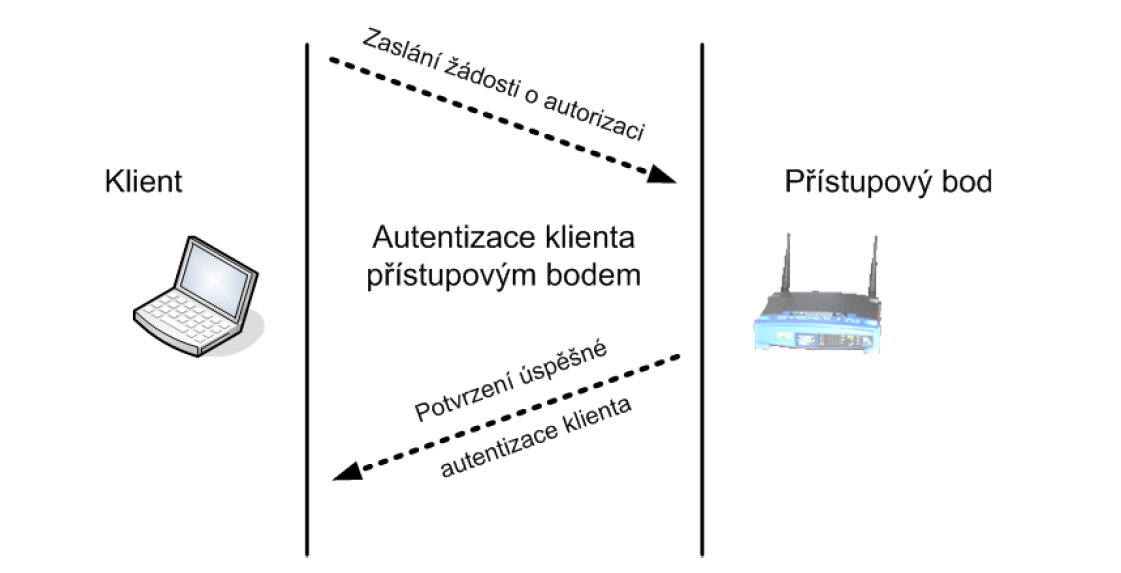
\includegraphics[scale=0.5]{images/OSA.png}
  \end{center}
  \caption[Autentizace klienta přístupovým bodem]{Autentizace klienta přístupovým bodem}
\end{figure}
\textbf{Shared Key Authentication} Metoda musí pracovat s algortimem WEP, která využívá klíče na straně klienta i na straně přístupového bodu. Pro správnou funkci musí být klíče stejné na obou stranách.
\begin{description}
    \item [Proces autentizace] \hfill \\
    Klient pošle přístupovému bodu žádost o autentizaci. \par
    AP vygeneruje náhodný text a zašle ho klientovi. \par
    Klient zašifruje přijatý řetězec svým WEP klíčem. \par
    -- V zašifrovaném tvar ho zašle zpět přístupovému bodu. \par
    AP dešifruje řetězec svým WEP klíčem. \par
    -- Vyhodnotí shodu původního a dešifrovaného řetězce. \par
    AP může ověřit, zda klient používá správný WEP klíč. \par
    -- Když ano, proces ověření klienta skončí úspěšně. \par
    -- Když ne, žádost klienta je odmítnuta. \par
    Oznámení o výsledku rozhodnutí: Authentication response. \par
\end{description}
\begin{figure}[ht]
\centering
  \begin{center}
    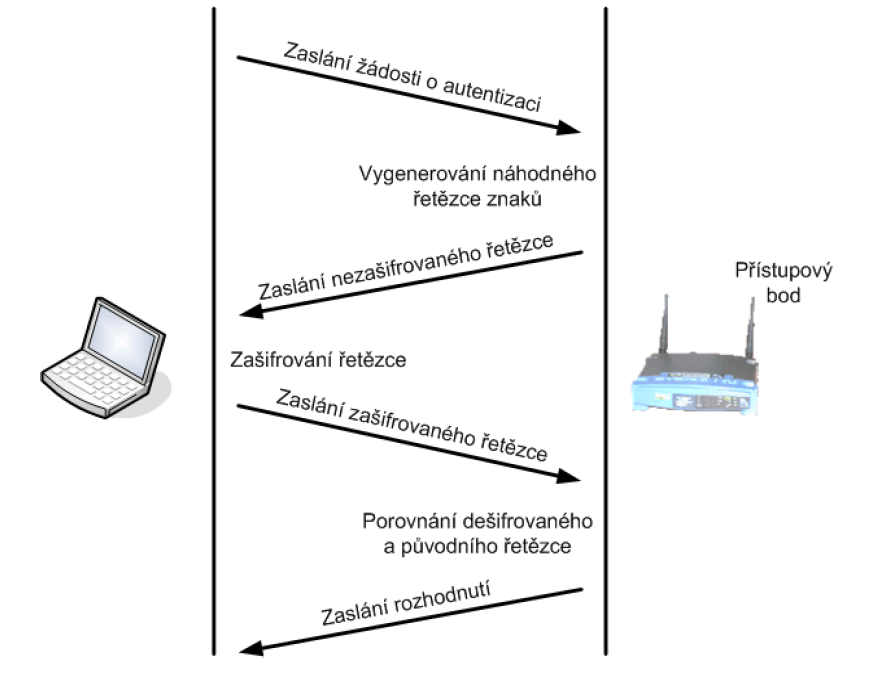
\includegraphics[scale=0.5]{images/SKA.png}
  \end{center}
  \caption[Autentizační metoda Shared Key Authentication]{Autentizační metoda Shared Key Authentication}
\end{figure}
Při \textbf{Shared Key Authentication} je možné odvodit WEP klíč díky zasílání otevřeného a zašifrovaného řetězce. Zabezpečení přenosu dat nebude účinné. Při \textbf{Open System Authentication} je obtížnější odhalení WEP klíče, který je použit pouze pro přenos dat.
\subsection{Asociace}
\begin{itemize}
    \item Druhý krok připojení klienta od WLAN
    \item Po asociaci klient může posílat data přes WLAN
    \item Inicializuje klient vysláním žádosti: association request
    \item AP žádost přijme nebo odmítne: assicoation response.
\end{itemize}
\subsection{Stav připojení}
Řízení přístupu CSMA/CA metodami: PCF a DCF. Přenost dat.
\subsection{Reasociace}
Obnovení spojení z důvodu ztráty spojení nebo kvůli velkému provozu v síti.
\begin{description}
    \item [Obnova spojení] \hfill \\
    Klient vyšle zprávu reassociation request. \par
    Přístupový bod odpovídá zprávou reassociatino response. \par
    \item[Vybudování nového spojení] \hfill \\
    Klient ruší spojení s aktuálním AP: disassociation request. \par
    Klient požádá o asociaci nový AP reassociation request -- reassociation response. \par
\end{description}
\subsection{Roaming}
Přecházení uživatelů mezi přístupovými body. Probíhá na druhé nebo třetí vrstvě. Na druhé vrstvě se uživatel přesunuje od jednoho přístupového bodu k druhému v rámci téže IP sítě / podsítě. Tj. jenom fyzické předání uživatelů mezi dvěma přístupovými body (handover). Pokud se přesouvá do jiné IP sítě, nemůže nadále používat nadále na venek používat původní IP adresu. K tomu je potřeba Mobile IP. Řeší tento problém pomocí domácí adresy, která je neměnná a cizí adresy, kterou si klient půjčuje v navštívených sítích.




\newpage
\section{Deterministické a náhodné přístupové metody využívané v sítích WLAN.}
\subsection{CSMA/CA}
\begin{itemize}
\item Kolize
\begin{itemize}
    \item Sdílené medium 
    \item Náhodný přístup
    \item U WLAN sítí je obtížné detekovat kolizi, proto se jí snaží jen vyhnout
\end{itemize}

  
\item Přístupová metoda 
\begin{itemize}
    \item Využívá zpětné potvrzování přijatých datových rámců 
    \item Snižuje efektivitu systému 
    \item Využívá náhodné čekací doby v případě, že medium není volné
\end{itemize}
\end{itemize}



\subsection{Náhodna přístupova metoda}
\subsubsection{Distribuovaná koordinační funkce (DCF – Distributed Coordination Function) }
\begin{itemize}
    \item Specifikována v standardu 802.11 
    \item Lze využít v BSS, ESS i IBSS 
    \item Využívá náhodnou přístupovou metodu
    \item Stanice soutěží o přístup k médiu: 
    \begin{itemize}
    \item stanice si vygenerují náhodné číslo
    \item každá stanice postupně snižuje svoje náhodné číslo každým hodinovým impulzem
a na konci hodinového impulzu zkontrolují obsazenost média
    \item Po uplynutí náhodně generovaného čekacího intervalu = Dosažení hodnoty 0 =>
zahájení vysílání
    \item Ostatní stanice zjistí, že medium už není volné a přestanou odpočítávat.
Zapamatování aktuální hodnoty u ostatních stanic - Využití během následujícího
soutěžení
    \item Po příjmu cílový uzel musí zkontrolovat přijatý rámec a zpětně potvrdit správný
příjem rámcem ACK
    \end{itemize}
\end{itemize}
\begin{figure}[ht]
\centering
  \begin{center}
    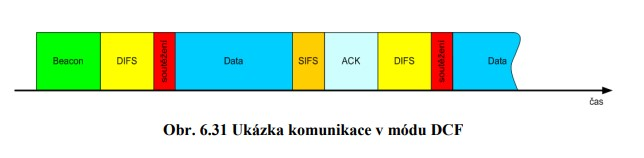
\includegraphics[scale=0.9]{images/dcf.jpg}
  \end{center}
\end{figure}

\subsection{Deterministicka přístupova metoda}
\subsubsection{Centralizovaná koordinační funkce (PCF - Point Coordiantion Fuction) }
\begin{itemize}
    \item Přístupová metoda bez soutěžení – řízená tj. deterministická
    \item AP pravidelně dotazuje stanic a zjišťuje, zda nemají data k vysílání
    \item Vhodné pro zajištění QoS
    \item Vyžaduje přítomnost AP
    \item Před využitím PCF musí klient nejdĜív sdělit AP, že umí odpovídat na dotazy
    \item Musí pracovat v kombinaci s DCF = Využíva Superrámec
    \item Průběh komunikace PCF:
    \begin{itemize}
    \item Proces je zahájen vysláním rámce „beacon“ 
    \item Interval bez soutěžení (Contention-Free Period - CFP)
    \begin{itemize}
    \item Řízení přístupu PCF – dotazování
    \item Zprávy CF-Poll – CF-ACK
    \item Ukončí AP zprávou CF-End
    \end{itemize}
    \item Nasleduje Interval soutěžení (Contention Period - CP) podle DCF 
     \begin{itemize}
     \item Využívá DCF (soutěžení stanic o přístup k médiu)
     \item První stanice, která získá přístup k médiu odešle svůj datový rámec
     \item Cílová stanice, resp. přístupový bod počká SIFS a pošle rámec ACK
     \item Příjem ACK znamená, že data byla doručena bez problémů
     \item Následuje další komunikace, zahájena příslušnou mezirámcovou mezerou
     \end{itemize}
    \end{itemize}
\end{itemize}
\begin{figure}[ht]
\centering
  \begin{center}
    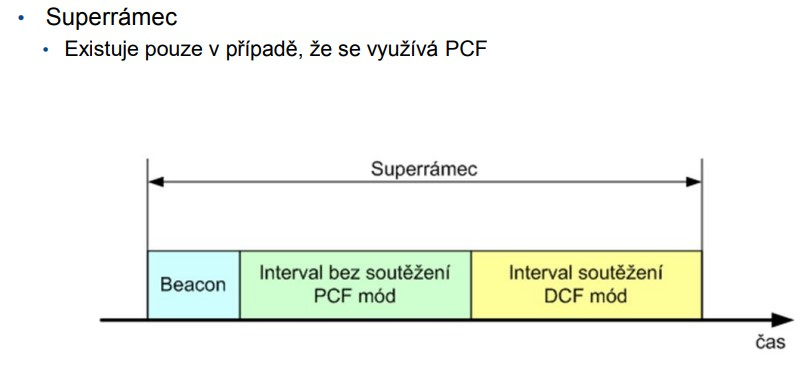
\includegraphics[scale=0.7]{images/superramec.jpg}
  \end{center}
\end{figure}


\newpage
\section{Vlastnosti základních algoritmů výběru buněk (PIM, iRRM, SLIP, DRRM).}
\subsection{PIM algoritmus}
Algoritmus Paralell Iterative Matching -- PIM využívá mechanizmus náhodného výběru. Buňky vstupující do propojovacího uzlu jsou uloženy do front VOQ a výběr proběhne iteračním procesem. Každý iterační krok je složen ze tří fází. Na začátku není žádný ze výstupních a výstupních portů označen a jen výstupní a výstupní porty, které budou neoznačeny, mohou vstoupit do následujícího iteračního kroku. Zmíněné tří fáze iteračního kroku jsou následující:
\begin{itemize}
    \item Inicializace\par
    \item Požadavky\par
    \item Potvrzení\par
    \item Výěr\par
    \item Přidělení páru vstup -- výstup\par
\end{itemize}
\begin{description}
  \item[Inicializace] \hfill \\
  Žádný ze vstupních a výstupních portů není označen.\par
  Neoznačené vstupní a výstupní porty mohou vstoupit do iteračního procesu.
  \item[Požadavky] \hfill \\
  Žádost od neoznačených vstupních portů.\par
  Všem výstupním portům, pro které mají buňky.
  \item[Potvrzení] \hfill \\ 
  Neoznačený výstupní port přijme více žádostí.\par
  Vyhoví pouze jedné z nich. \par
  Náhodný výběr -- stejná pravděpodobnost výběru pro všechny žádosti.\par
  Oznámení výsledku výběru vstupnímu portu (= samo potvrzení).
  \item[Výběr] \hfill \\
  Vstupní port může dostat více potvrzení.\par
  Vybere výstup náhodně.
  \item[Přidělení páru vstup -- výstup] \hfill \\
  Vybrané vstupní a výstupní porty se stanou označenými.\par
  Nebudou zahrnuty do dalšího iteračního kroku.\par
\end{description}
Průběh jednoho iteračního kroku je znázorněn na obrázku níže. V každém iteračním kroku je pak označeno průměrně 75\% potvrzení. Iterace konverguje poměrně rychle, během $O(logN)$ iteračních kroků. Nevýhoda je náročná implementace rychlých náhodných funkcí. V případě rovnoměrného provozu dosahuje algoritmus PIM propustnost 63\% pro 1 a 100\% pro N iteračních kroků.
\begin{figure}[ht]
\centering
  \begin{center}
    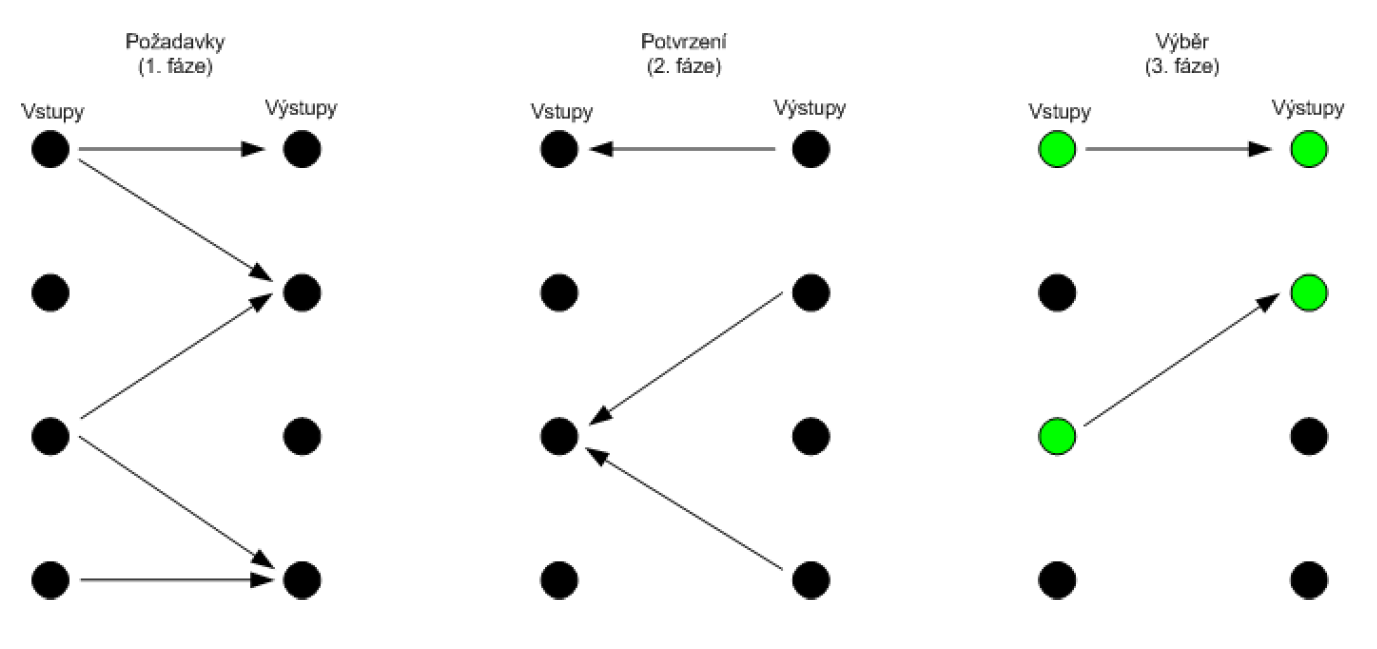
\includegraphics[scale=0.5]{images/PIM.png}
  \end{center}
  \caption[Jeden iterační krok algoritmu PIM)]{Jeden iterační krok algoritmu PIM}
\end{figure}
\subsection{iRRM algoritmus}
Iterative Round -- Robin Matching, podobný algoritmu PIM. Místo náhodného výběru využívá mechanizmu round -- robin a to jak u výstupního, tak u vstupního portu. Každý arbiter (řídící model) spravuje ukazatel ukazující na port, který má v daném časovém okamžiku nejvyšší prioritu. U vstupního portu se ukazatel nazývá \textbf{accept pointer} a u výstupního portu se nazývá \textbf{grant pointer}.Na obrázku níže je znázorněn ukazatel u 4 -- portového propojovacího uzlu.
\begin{figure}[ht]
\centering
  \begin{center}
    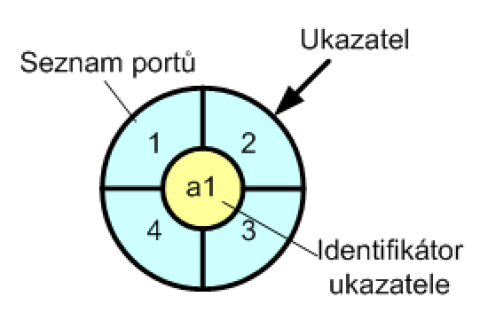
\includegraphics[scale=0.5]{images/iRRM.png}
  \end{center}
  \caption[Ukazatel algoritmu round -- robin]{Ukazatel algoritmu round -- robin}
\end{figure}
\subsubsection{Popis procesu}
\begin{description}
  \item[Inicializace] \hfill \\
  Žádný ze vstupních a výstupních portů není označen.\par
  \item[Iterace] \hfill \\
  Žádost od neoznačených vstupních portů.
  \begin{itemize}
      \item Všem vstupním portům, pro které mají buňky.\par
  \end{itemize}
  Neoznačený výstupní port přijme více žádostí
  \begin{itemize}
      \item Vybere žádost od vstupu s nejvyšší prioritou.\par
      \item Příp. od nejbližšího následujícího portu v seznamu. \par
  \end{itemize}
  Oznámení výsledku výběru.
 \begin{itemize}
    \item Výstupy informují vybrané vstupní porty. \par
    \item Informují také nevybrané vstupní porty. \par
  \end{itemize}        
  Nastavení ukazatele arbitru.
  \begin{itemize}
    \item Na port následující hned za právě vybraným. \par
    \item Výstupy, které nedostaly žádost -- ukazatel zůstane v původním stavu. \par
  \end{itemize}
  Pokud vstupní port obdrží více potvrzení
  \begin{itemize}
      \item Výběr potvrzení. \par
      \item Od výstupního portu s právě největší prioritou. \par
      \item příp. od nejbližšího následujícího portu v seznamu. \par
  \end{itemize}
  Aktualizace ukazatele vstupního arbiteru
  \begin{itemize}
      \item Na port následující hned za právě vybraným. \par
      \item Vstupy, které neposlaly žádost, ukazatel nemění. \par
  \end{itemize}
\end{description}
\subsubsection{Příklad algoritmu iRRM}
\begin{figure}[ht]
\centering
  \begin{center}
    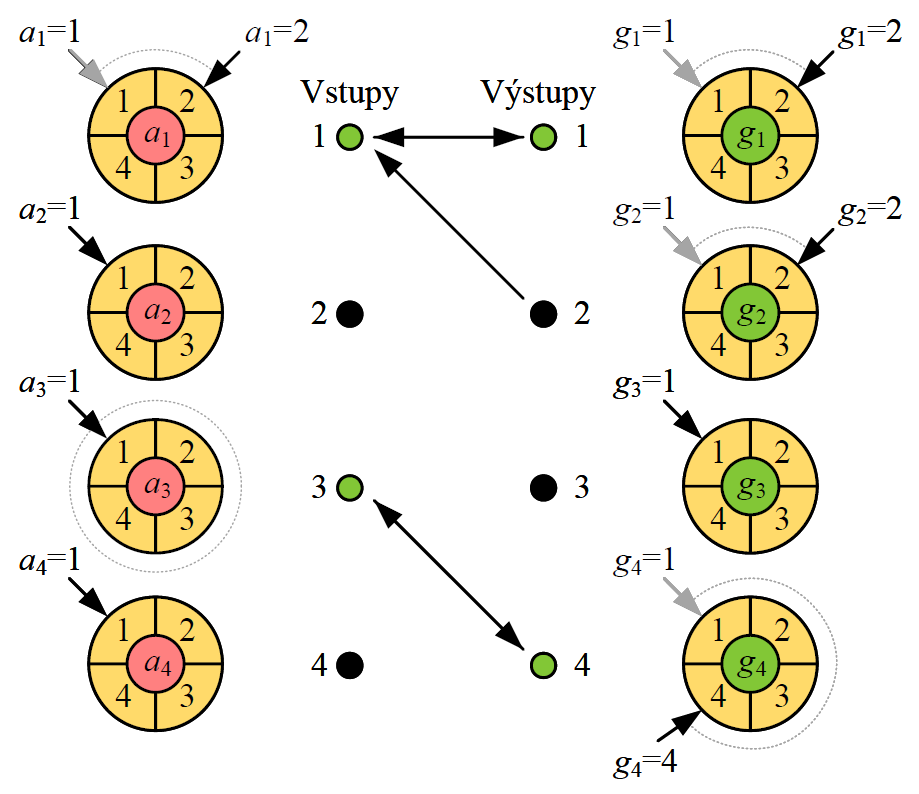
\includegraphics[scale=0.5]{images/iRRM_priklad.png}
  \end{center}
  \caption[Příklad algoritmu iRRM]{Příklad algoritmu iRRM}
\end{figure}
\begin{description}
  \item[Inicializace] \hfill \\
  \begin{equation}
      a_i = g_i = 1, pro \,\,\, i = 1, 2, 3, 4
  \end{equation}
  \item [Žádost od neoznačených vstupních portů] \hfill 
  \item [Oznámení výsledku výběru] \hfill \\
  \begin{equation}
      g_1 = 1 + 1, g_2 = 1 + 1, g_3 = 1\,\,\, a \,\,\, g_4 = 3 + 1
  \end{equation}
  \item [Výběr potvrzení a aktualizace ukazatele vstupního arbiteru] \hfill \\
\begin{equation}
    a_+ = 1 + 1, a_3 = mod_4{(4+1)} = 1
\end{equation}
\end{description}
\subsection{iSLIP algoritmus}
Zdokonalení algoritmu iRRM, došlo ke aktualizaci výstupního portu (grant pointer) a to pouze v případě, pokud je dané potvrzení akceptováno. Vybraná dvojice vstupního a výstupního portu bude mít vždy nejnižší prioritu. Spravedlivé přidělování šířky pásma datovým tokům a 100 \% propustnost.
\subsection{Kroky iteračního procesu}
\begin{description}
  \item [Inicializace] \hfill \\
  Žádný vstupní ani výstupní port není označen. \par
  \item [Žádost od neoznačených vstupních portů] \hfill \\
  Všem výstupním portům, pro které mají buňky. \par
  \item [Neoznačený výstupní port přijme více žádostí] \hfill \\
  Vybere žádost od vstupu s nejvyšší prioritou. \par
  Příp. od nejbližšího následujícího portu v seznamu. \par
  \item [Oznámení výsledku výběru] \hfill \\
  Výstupy informují vybrané vstupní porty. \par
  Informují také nevybrané vstupní porty. \par
  Výstup zatím neaktualizuje ukazatele arbiteru. \par
  \item [Pokud vstupní port obdrží více potvrzení] \hfill \\
  Výběr potvrzení. \par
  Od výstupního portu s právě největší prioritou. \par
  Příp. od nejbližšího následujícího portu ze seznamu. \par
  \item [Aktualizace ukazatele $a_i$ vstupního arbitru] \hfill \\
  Na port následující hned za právě vybraným výstupem. \par
  Pouze v prvním iteračním kroku. \par
  \item [Aktualizace ukazatele $g_i$ výstupního arbitru] \hfill \\
  Na port následující hned za vstupním portem v seznamu, který akceptoval potvrzení. \par
  Pouze v prvním iteračním kroku. \par
\end{description}
\subsection{Příklad iSLIP}
\begin{figure}[ht]
\centering
  \begin{center}
    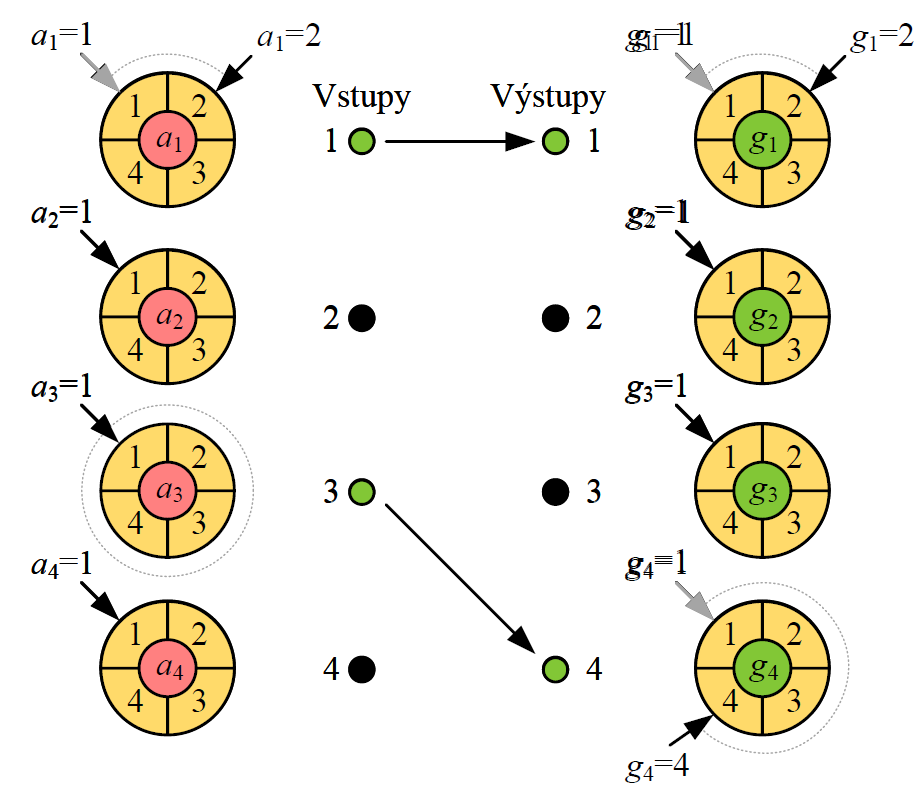
\includegraphics[scale=0.5]{images/iSLIP_priklad.png}
  \end{center}
  \caption[Příklad algoritmu iSLIP]{Příklad algoritmu iSLIP}
\end{figure}
\begin{description}
  \item[Inicializace] \hfill \\
  \begin{equation}
      a_i = g_i = 1, pro \,\,\, i = 1, 2, 3, 4
  \end{equation}
  \item [Žádost od neoznačených vstupních portů] \hfill 
  \item [Oznámení výsledku výběru] \hfill 
  \item [Výběr potvrzení a aktualizace ukazatele vstupního arbiteru] \hfill \\
  \begin{equation}
    a_+ = 1 + 1, a_3 = mod_4{(4+1)} = 1
  \end{equation}
  \item [Aktualizace ukazatele výstupního arbiteru] \hfill \\
  \begin{equation}
      g_1 = 1 + 1, g_4 = 3 + 1
  \end{equation}
\end{description}
\subsection{DRRM algoritmus}
Dual Round -- Robin Matching implementuje mechanizmus Round -- Robin a využívá systém virtuálních front VOQ. Vstupní port se skládá z VOQ front a vstupního arbitru. Výstupní port obsahuje pouze výstupní arbitr.
\begin{description}
  \item [Výběr žádosti] \hfill \\
  Řídí vstupní arbiter. \par
  Využitím mechanizmu Round -- Robin. \par
  Výběr VOQ fronty, která obsahuje buňky k odeslání. \par
  \item [Zaslání žádostí] \hfill \\
  Každý vstup na příslušný výstupní port. \par
  \item [Výběr jednoho požadavku] \hfill \\
  Provede výstupní arbiter. \par
  Využije mechanizmus Round -- Robin. \par
  \item[Zaslání potvrzení] \hfill
  \item [Aktualizace ukazatele vstupních portů] \hfill \\
  Puouze z vybraných vstupů. \par
  \item [Aktualizace ukazatele výstupních portů] \hfill \\
  Pouze u dotázaných. \par
  \subsection{DRRM příklad}
\end{description}
\begin{figure}[ht]
\centering
  \begin{center}
    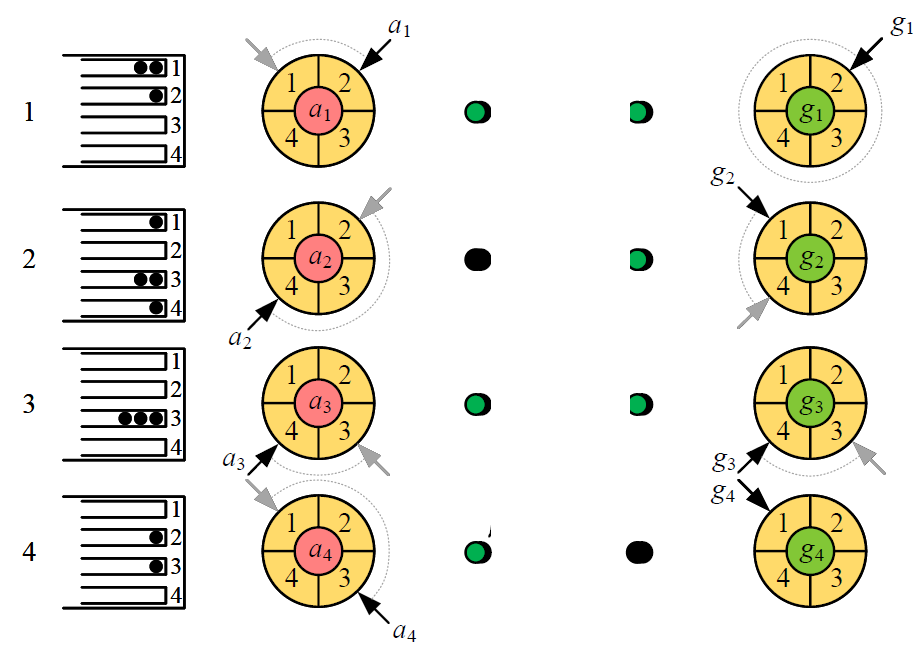
\includegraphics[scale=0.5]{images/DRRM_priklad.png}
  \end{center}
  \caption[Příklad algoritmu DRRM]{Příklad algoritmu DRRM}
\end{figure}
\begin{description}
\item [Odeslání žádostí] \hfill
\item [Potvrzení a vytvoření párů vstup -- výstup] \hfill
\item [Aktualizace vstupních a výstupních arbitrů] \hfill \\
\begin{equation}
    a_1 = 2, a_2 = 4, a_3 = 4, a_4 = 3
\end{equation}
\begin{equation}
    g_1 = mod_4{(2+4)} = 2, g_2 = mod_4{(4+1) = 1}, g_3 = 4, g4 = g_4
\end{equation}
\end{description}
\subsection{Desynchronizační efekt}
Desynchronizační efekt:
\begin{itemize}
    \item Vstupní arbitry žádají o různé výstupy
    \item Větší propustnost
    \item Příklad -- jsou zobrazeny pouze první buňky z vybrané VOQ fronty
\end{itemize}
\begin{figure}[ht]
\centering
  \begin{center}
    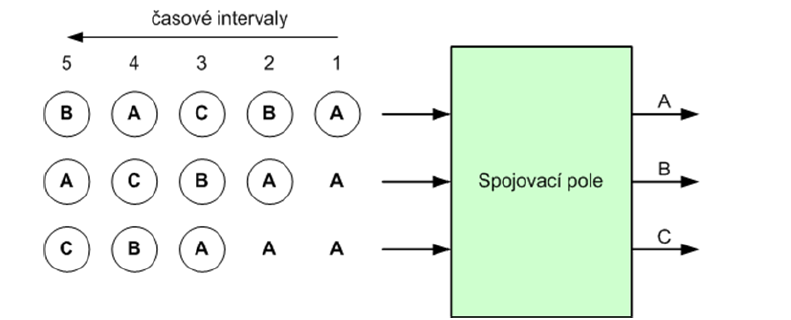
\includegraphics[scale=0.6]{images/DRRM_desyn.png}
  \end{center}
  \caption[Desynchronizační efekt]{Desynchronizační efekt}
\end{figure}
Projevuje se u DRRM i iSLIP, DRRM je výhodnější -- kratší výměna informací - větší rychlost.

\newpage
\section{Vlastnosti a struktura přepínače se sdíleným mediem a se sdílenou pamětí.}
\subsection{Prepináč so zdieľaným médiom}
Vstupné porty prepínačov tohto typu sú pripojené k zdieľanému médiu pomocou
časového multiplexu. V prípade, že $N$ je počet portov, časový interval, zodpovedajúci \textbf{bunkovej perióde}, je rozdelený na $N$ mini intervalov, z ktorých každý prislúcha jednému z vstupných portov. Daný port počas tohto mini intervalu môže zapísať svoje dáta na zdieľané médium (zbernica alebo kruh). Pretože je médium zdieľané medzi $N$ portami, musí byť šírka pásma zdieľaného média N-krát vyššia, než je šírka pásma vstupného rozhrania. Z toho vyplýva, že priepustnosť zdieľaného média určuje kapacitu prepínača. Charakteristická architektúra takého prepínača je na Obr.12. Každá výstupná linka je pripojená na zdieľané vysokorýchlostné médium cez adresný filter a vyrovnávaciu pamäť typu FIFO. K bunke je bežne pripojená ešte \textbf{hlavička}, ktorá obsahuje
bitovú mapu výstupných portov. Nastavením bitu príslušného odchádzajúceho portu je potom signalizované, že bunka je určená pre tento odchádzajúci port. Adresný filter overuje túto bitovú mapu buniek objavujúcich sa na zdieľanom médiu, a v prípade splnenia kritérií filtrovania, \textbf{bunku skopíruje do vyrovnávacej pamäte}. \newline
Ďalším obmedzením môže byť rýchlosť zápisu do vyrovnávacej pamäte, kedy vyrovnávacia pamäť musí byť schopná zapísať až $N$ buniek za jeden časový interval (z každého vstupu smeruje prevádzka na jeden výstup).Riadenie prepínača je \textbf{decentralizované} a preto každý výstupný port môže pracovaťnezávisle na ostatných. S nezávislosťou jednotlivých portov súvisí \textbf{menšia efektivita} využívania hardvérových prostriedkov, ktoré nie sú zdieľané medzi odchádzajúce porty. Môže tak vzniknúť situácia, že jeden z výstupných portov už zahadzuje bunky, pretože má preplnenú vyrovnávaciu pamäť, pričom ostatné vyrovnávace pamäte môžu byť úplne prázdne. Prepínače so \textbf{zdieľaným médiom} sa často využívajú aj v telekomunikačných systémoch, kde je \textbf{šírka pásma} vstupných liniek pomerne {malá}.

\begin{figure}[ht]
\centering
  \begin{center}
    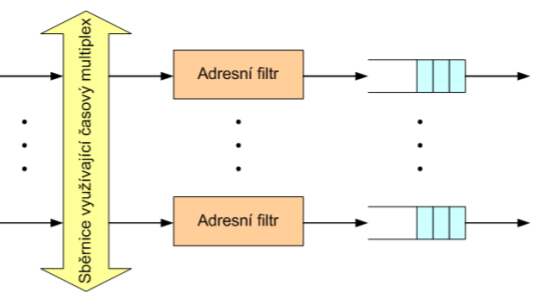
\includegraphics[scale=0.8]{images/zdiel_medium.png}
  \end{center}
  \caption[Architektúra prepínača so zdieľaným médióm]{Architektúra prepínača so zdieľaným médióm}
\end{figure}

\newpage
\subsection{Prepínač so zdieľanou pamäťou}
Pri tomto type prepínača sú prichádzajúce bunky radené do \textbf{časového multiplexu} a sú postupne zapisované do zdieľanej pamäťovej oblasti. Prepájanie je potom realizované čítaním buniek vo forme multiplexovaného toku dát, ktorý je potom demultiplexovaný a vedený k jednotlivým výstupom. Riadenie zápisu a čítania z pamäte vykonáva modul riadenia na základe informácií získaných z hlavičky buniek. Ukážka architektúry prepínača so zdieľanou pamäťou je na Obr.13.Prepínače so zdieľanou pamäťou vykazujú \textbf{najlepšie využitie prostriedkov}, pretože všetky vstupné aj výstupné porty zdieľajú jednu pamäťovú oblasť. Toto riešenie tiež umožňuje jednoduché prispôsobenie veľkosti pamäte k požiadavkám na stratovosť.Rýchlosť operácií s pamäťou je rovnako N-krát vyššia, než rýchlosť linkových rozhraní. Preto rýchlosti pamäte priamo obmedzujú kapacitu prepínača. Ďalšou nevýhodou je zložité riadenie zápisu a čítania z pamäte.\newline


Existujú \textbf{dve metódy zdieľania pamäťového priestoru medzi portami}:
\begin{enumerate}
    \item Úplne rozdelenie -- pamäťový priestor je rozdelený na $N$ rovnakých častí, kde každá dielčiačasť je priradená jednému zo vstupných portov a bunka je následne zapísaná do pamäte podľa toho, pre ktorý výstupný port je určená
    \item Plné zdieľanie -- celý pamäťový priestor je zdieľaný všetkými vstupnými portami, čo je efektívnejším využítim pamäte, musia však existovať algoritmy, ktoré skúmajú využitie pamäte jednotlivými portami a zabraňuju monopolizácií
\end{enumerate}

\begin{figure}[ht]
\centering
  \begin{center}
    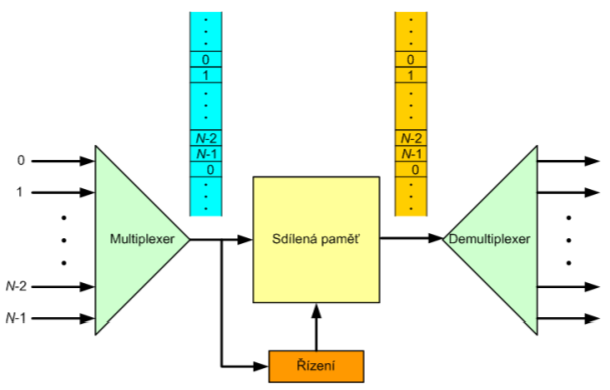
\includegraphics[scale=0.8]{images/zdiel_pamat.png}
  \end{center}
  \caption[Architektúra prepínača so zdieľanou pamäťou]{Architektúra prepínača so zdieľanou pamäťou}
\end{figure}

\newpage
\section{Struktura spojovacích polí s prostorovým dělením kanálu (křížový přepínač, plně propojená struktura, Banyan).}
Pri tejto skupine prepináčov existuje \textbf{viac ciest} medzi prichádzajúcimi a odchádzajúcimi portami. Je možné ich využiť na súčasný prenos viacerých buniek. Tým je dosihanuté, že \textbf{priepustnosť prepojovacieho uzla} je násobkom šírky pásma ciesty a počtu ciest, ktoré súčasne prenášajú bunky. Prakticky je kapacita prepínača obmedzená faktormi, ktoré súvisia s fyzickou implementáciou, napr. vývod súčiastok či problém so synchronizáciou. Viaccestné prepínače sú odolnejšie vočí poruchám, jednocestné zase jednoduchšie na implementáciu.

\subsection {Krížový prepínač}
Prepojovací uzol vyžaduje krížový prepináč so štruktúrou $N*N$, obsahujúci $N^2$ samostatne riadených spínacích prvkov,každý odpovedá dvojici vstup--výstup. Každý spínací prvok má \textbf{dva stavy}, a to, rozopnutý stav , ktorý je továrenský a zopnutý stav.
Spojenie medzi vstupným portom a výstupným je dosiahnuté uvedením spínacieho prvku do zopnutého stavu. Je možné spúšťať u každého spínacieho prvku uvedenie do zopnutého stavu automaticky príchodom bunky. Proces prebieha nezávislo na ostatných bunkách. Pole sa tak stáva \textbf{samosmerovacím} -- riadiace funkcie sú distribuované medzi spínacie prvky.Výhodou tejto architektúry je nemožnosť vnútorného blokovania, jej modulárnosť a jednoduchosť. Obmedzením je však narastanie spínacích uzlov kvadraticky. Rozhodovanie o výbere bunky pre daný port a časový interval sú častým úzkym miesto väčšieho spojovacieho poľa.Na obrázku 14 je znázornený krížový prepínač,kde vodorovné linky značia vstupy a zvislé výstupy.

\begin{figure}[ht]
\centering
  \begin{center}
    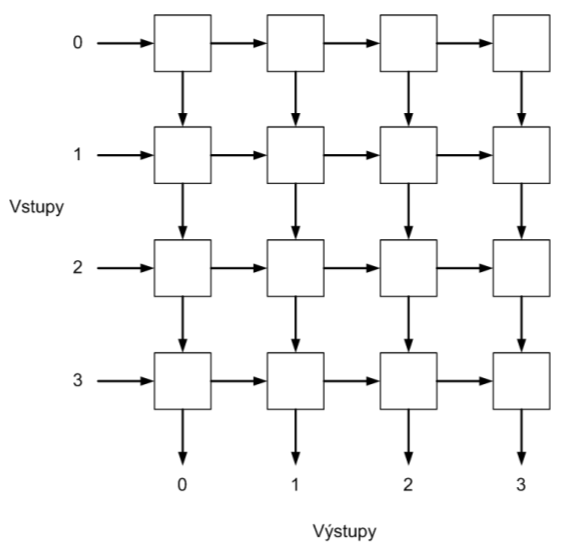
\includegraphics[scale=0.8]{images/kriz_prep.png}
  \end{center}
  \caption[Krížový prepínač]{Krížový prepínač}
\end{figure}

\subsubsection{Vyrovnávacia pamäť v spínacích prvkoch}
V každom spínacom bode sa nachádza adresný filter, ktorý bunky s cieľovou adresou odpovedajúcej príslušnému výstupnému portu prepúšťa do vyrovnávacej pamäte. Z buniek, ktoré čakaú vo vyrovnávacej pamäti je nutné vybrať, ktorá bunka v ktorom časovo okamihu môže byť prenesená na výstup. Architekrúra netrpí blokovaním fronty. Výstupný buffer portu je rozdelený na $N$ menších pamätí. Nie je využité zdieľanie pamätí, preto je nutné využitie viac pamätí pre danú veľkosť stratovosti. Nevýhodou je taktiež technologické riešenie,pretože pamäte musia byť integrované spolu s riadiacou logikou spojovacieho poľa do jedného čipu, tým je obmedzený počet spínacích prvkov.


\begin{figure}[ht]
\centering
  \begin{center}
    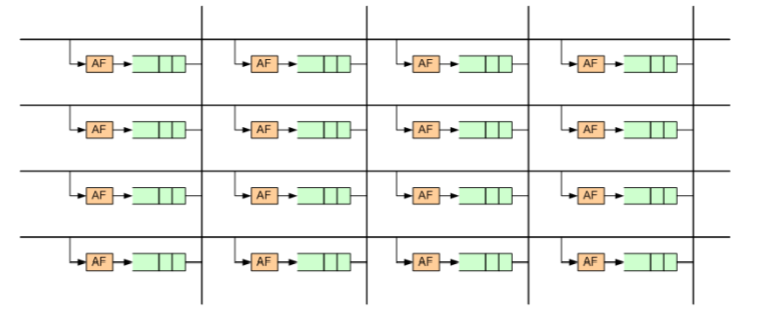
\includegraphics[scale=0.8]{images/kriz_prep_spin.png}
  \end{center}
  \caption[Krížový prepínač s vyrovnávacou pamäťou v spínacích prvkoch]{Krížový prepínač s vyrovnávacou pamäťou v spínacích prvkoch}
\end{figure}

\subsubsection{Vyrovnávacia pamäť na vstupe}
Prijatá bunka je najprv uložená do vstupnej vyrovnávacej pamäte a čaká, aby mohla vstúpiť do spojovacieho poľa. V prípade konfliktov o prístup na rovnaký výstupný port ,ktoré sú riešené distribuovane sa algoritmus výberu robí zvlášť v každom spínacom bode. Keď sa bunka dostane k spínaciemu miestu, pre daný vstupný port je to oznámené blokačným signálom. Následne výstupný port preruší vysielanie bunky a nechá ju vo vyrovnávacej pamäti. V prípade centralizovaného výberu buniek pre každý výstupný port zvlášť prebehne výber tak, aby bola pre každý port len jedna bunka.

\begin{figure}[ht]
\centering
  \begin{center}
    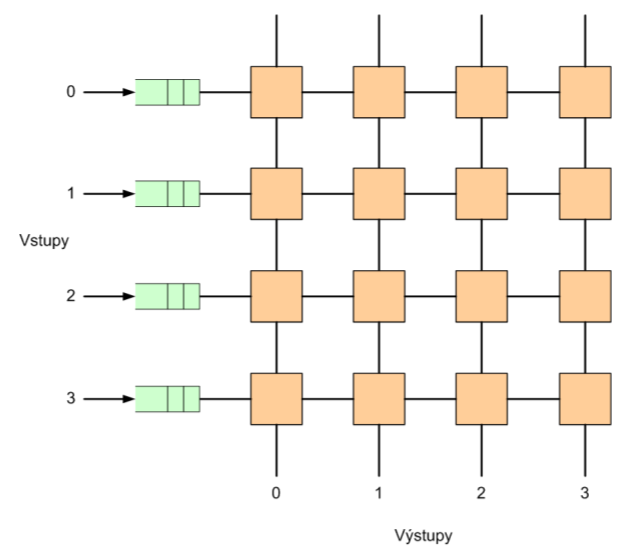
\includegraphics[scale=0.5]{images/kriz_prep_vstup.png}
  \end{center}
  \caption[Krížový prepínač s vyrovnávacou pamäťou na vstupe]{Krížový prepínač s vyrovnávacou pamäťou na vstupe}
\end{figure}

\subsubsection{Vyrovnávacia pamäť na výstupe}
Veľmi podobné vlastnosti, ako v štruktúre s výrovnávacou pamäťou v spojovacom uzle.Zarovnanie pamäte portu vytvára jednu oblasť, čo prináša efektívnejšie využitie pamäte.


\subsection{Prepínač na plne prepojené štruktúry}
Tieto prepínače sa vyznačujú tým, že každý vstup ma samostatné spojenie s každým výstupom. Toto spojenie je dosiahnuté pomocou $N$ zberníc, kde každa zubernica vedie of konkrétneho vstupného portu ku všetkým výstupným portom. Spojovacie pole vyžaduje $N$ samostatných vyrovnávacích pamätí na výstupných portoch. Bunka je rozoslaná na každý vstupný port. Bunky od rôznych vstupných portov sú súčasne privedené na rovnaký výstupný port. Výstupný port tak robí filtrovanie buniek a ich ukladanie do vyrovnávacej pamäte. Každy port má vlastný filter buniek a vyrovnávaciu pamäť. Štruktúra je jednoduchá a neblokujúca.

\begin{figure}[ht]
\centering
  \begin{center}
    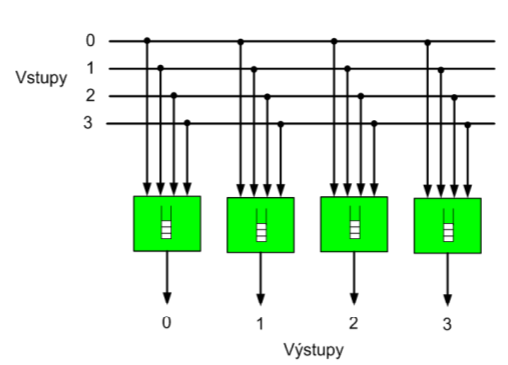
\includegraphics[scale=0.8]{images/plne_prep.png}
  \end{center}
  \caption[Prepínač na plne prepojené štruktúry]{Prepínač na plne prepojené štruktúry}
\end{figure}

\newpage
\subsection{Prepínáč na spojovacie pole typu Banyan}
Jedná sa o jednocestný a samosmerovací prepínač zostavený zo spínacích elementov 2x2.Poznáme 3 topológie -- Banyan, Delta, Omega.\newline
Počet spínacích elementov a ciest v tejto rodine spojovacích polí narastá $N$log$N$-krát, čo je v prípade veľkých spojovacích polí výrazne lepšie. Samosmerovací algoritmus nevyžaduje prídavný riadiaci modul a ako všetky spojovacie polia so zdieľaným médiom umožňuje paralelný prenos viacerých buniek. Samozrejme, táto štruktúra má aj niekoľko nevýhod. Najvýznamnejšia z nich je, že môže nastať vnútorné blokovanie a priepustnosť spojovacieho poľa rapídne klesá s nárastom veľkosti. Pokles priepustnosti je možné kompenzovať využitím spínacích prvkov MxM, kde M>2 namiesto prvkov 2x2. Napriek zvýšenej priepustnosti ale spojovacie pole zostane stále blokovacím.

\begin{figure}[ht]
\centering
  \begin{center}
    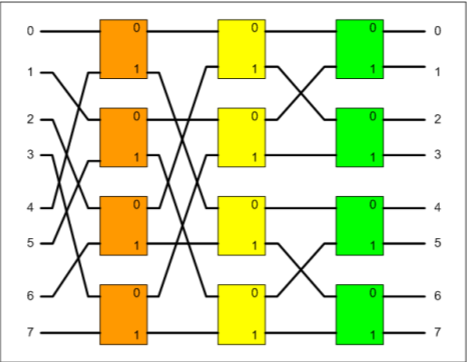
\includegraphics[scale=0.8]{images/banyan.png}
  \end{center}
  \caption[Prepínáč na spojovacie pole typu Banyan]{Prepínáč na spojovacie pole typu Banyan}
\end{figure}

\newpage
\section{Výhody a nevýhody architektur pro přepojovací uzly využívající: vstupní vyrovnávací paměti, výstupní vyrovnávací paměti, sdílenou paměť, a virtuální výstupní fronty.}

\subsection{Vstupná vyrovnávacia pamäť}
Najväčšou nevýhodou je možnosť blokovania rady, ktorá spôsobuje pokles priepustnosti v prípade veľkého prepináča až na hodnotu 58,6 $\%$. Pre zvýšenie priepustnosti je možné využiť systém okna, kedy je zo vstupného vyrovnávacieho portu vybraných viacero buniek určených pre potenciálne odoslanie. Prenesená však bude maximálne len jedna. Počet potencionálne prenositelných buniek určuje veľkosť okna. Zvýšením veľkosti okna na dve sa zvýši priepustnosť na 70 $\%$. Výhodou je ukladanie buniek vo vyrovnávacej pamäti.

\begin{figure}[ht]
\centering
  \begin{center}
    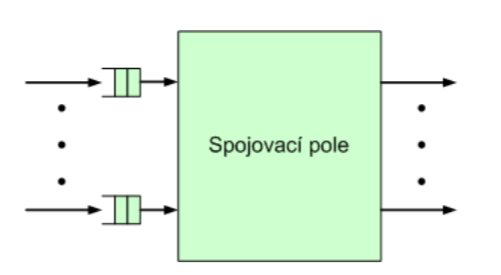
\includegraphics[scale=0.8]{images/propoj_vstup.png}
  \end{center}
  \caption[Štruktúra prepojovacieho uzla so vstupnou vyrovnávacou pamäťou]{Štruktúra prepojovacieho uzla so vstupnou vyrovnávacou pamäťou}
\end{figure}

\subsection{Výstupná vyrovnávacia pamäť}
Prepojovací uzol s výstupnou vyrovnávacou pamäťou umožňuje, aby každá bunka, ktorá vstúpi do spojovacieho poľa, bola doručená na požadovaný výstupný port, tj. priepustnosť tejto štruktúry je 100 $\%$. Výstupný port však môže prijať v jednej bunkovej perióde až $N$ buniek, čo kladie veľké nároky na rýchlosť spracovania a ukladanie buniek do vyrovnávacej pamäte portu.

\begin{figure}[ht]
\centering
  \begin{center}
    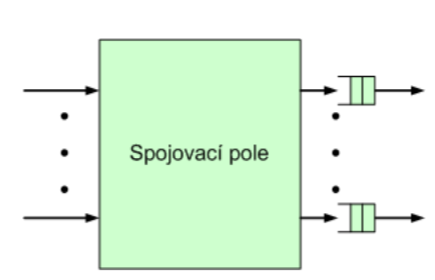
\includegraphics[scale=0.8]{images/propoj_vystup.png}
  \end{center}
  \caption[Štruktúra prepojovacieho uzla s výstupnou vyrovnávacou pamäťou]{Štruktúra prepojovacieho uzla s výstupnou vyrovnávacou pamäťou}
\end{figure}

\subsection{Zdieľaná pamäť}
Výhodou je vysoká priepustnosť, nízke oneskorenie a veľmi efektívne využitie pamäte hlavne pre menšie prepojovacie uzly.V prípade viacvrstvových štrukúr spojovanie viacerých spojovacích polí do jednej štruktúry vedie k zníženiu efektivity. Uloženie bunky do viacerých vyrovnávacích pamäti môže viesť k zmene poradia, čo je nutné eliminovať zložitým a drahým prídavným zariadením.

\begin{figure}[ht]
\centering
  \begin{center}
    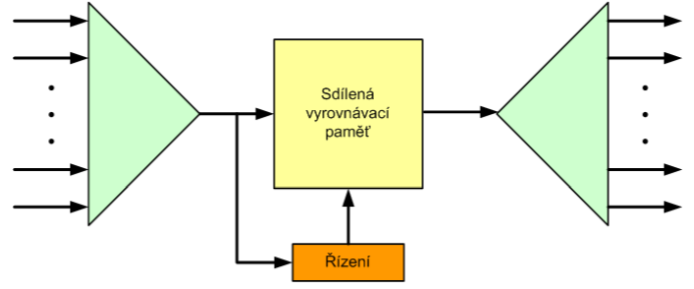
\includegraphics[scale=0.8]{images/propoj_zdiel.png}
  \end{center}
  \caption[Štruktúra prepojovacieho uzla so zdieľanou vyrovnávacou pamäťou]{Štruktúra prepojovacieho uzla so zdieľanou vyrovnávacou pamäťou}
\end{figure}

\subsection{Virtuálne výstupné rady}
Výhodou tohto uzla je predovšetkým eleiminácia blokovania rady, čo zabezpečuje zväčšenie priepustnosti celého uzla. Vstupná vyrovnávacia pmäť je rozdelená do $N$ logicky rozdelených rád a každá odpovedá jednému z výstupných portov. Nevýhodou je však zložité riadenie rád a potreba inteligentného výberu bunky pre vstup do spojovacieho uzla. Systém musí pracovať s $N*N$ virtuálnymi radami v každej bunkovej periódou.

\begin{figure}[ht]
\centering
  \begin{center}
    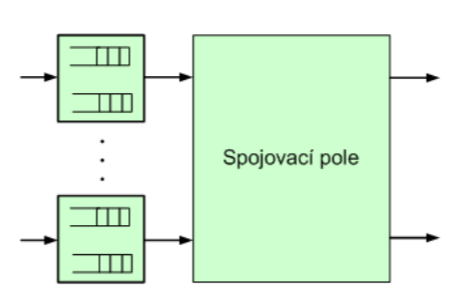
\includegraphics[scale=0.8]{images/propoj_virt.png}
  \end{center}
  \caption[Štruktúra prepojovacieho uzla s virtuálnou výstupnou radou]{Štruktúra prepojovacieho uzla s virtuálnou výstupnou radou}
\end{figure}

\end{document}
